\documentclass[aps,prx,reprint,amsmath,amssymb,superscriptaddress,longbibliography]{revtex4-2}

\usepackage[T1]{fontenc}
\usepackage{lmodern}
\usepackage{microtype}
\usepackage{bm}
\usepackage{mathtools}
\usepackage{amsthm}
\usepackage{graphicx}
\graphicspath{{figures/}}
\usepackage{booktabs}
\usepackage{array}
\usepackage{tabularx}
\usepackage{enumitem}
\usepackage{xcolor}
\usepackage{hyperref}
\usepackage[nameinlink,noabbrev]{cleveref}
\usepackage{tikz}
\usetikzlibrary{arrows.meta,positioning,fit,calc,shapes.geometric,backgrounds,decorations.pathreplacing}

\definecolor{linkblue}{RGB}{24,74,128}
\definecolor{sysblue}{RGB}{52,91,145}
\definecolor{envteal}{RGB}{63,134,128}
\definecolor{accentorange}{RGB}{202,119,54}
\definecolor{accentred}{RGB}{165,78,72}
\definecolor{softgray}{RGB}{242,244,247}
\definecolor{deepgray}{RGB}{75,82,92}
\hypersetup{
 colorlinks=true,
 linkcolor=linkblue,
 citecolor=linkblue,
 urlcolor=linkblue,
 pdftitle={Identifiability of Environmental Records in Quantum Darwinism: Learning Readouts from Redundancy and Intervention},
 pdfauthor={Marwan AIT HADDOU}
}

\newtheorem{theorem}{Theorem}
\newtheorem{proposition}{Proposition}
\newtheorem{lemma}{Lemma}
\newtheorem{corollary}{Corollary}
\newtheorem{definition}{Definition}
\newtheorem{remark}{Remark}

\newcommand{\tr}{\operatorname{Tr}}
\newcommand{\supp}{\operatorname{supp}}
\newcommand{\TV}{\operatorname{TV}}
\newcommand{\rank}{\operatorname{rank}}
\newcommand{\Herm}{\operatorname{Herm}}
\newcommand{\sign}{\operatorname{sign}}
\newcommand{\diag}{\operatorname{diag}}
\newcommand{\Span}{\operatorname{span}}
\newcommand{\eps}{\varepsilon}
\newcommand{\cH}{\mathcal H}
\newcommand{\cS}{\mathcal S}
\newcommand{\cM}{\mathcal M}
\newcommand{\cX}{\mathcal X}
\newcommand{\cZ}{\mathcal Z}
\newcommand{\ketbra}[1]{|#1\rangle\!\langle #1|}

\begin{document}


\title{\texorpdfstring{Identifiability of Environmental Records in Quantum Darwinism:\\Learning Readouts from Redundancy and Intervention}{Identifiability of Environmental Records in Quantum Darwinism: Learning Readouts from Redundancy and Intervention}}

\author{Marwan AIT HADDOU}
\email{aithaddou.marwan@outlook.com}
\affiliation{Independent Researcher, Morocco}
\thanks{ORCID: \href{https://orcid.org/0009-0008-1734-1721}{0009-0008-1734-1721}}

\date{August 16, 2026}

\begin{abstract}
Quantum Darwinism explains how pointer information becomes redundantly accessible through environmental fragments. We study the inverse problem in which those records exist but the local readout convention is unknown. We separate three targets: identifying a decoder, identifying the latent record ensemble, and assigning the recovered record to the designated system. For equal-prior binary records of arbitrary finite dimension, two fragments determine the local Helstrom contrast directions from the rank-one connected environmental operator; a known unequal prior already admits exact counterexamples. For multiclass records, two-fragment data determine a discriminant operator subspace, while a third generic view or structured spectrum-broadcast support can provide stronger recovery. Product redundancy improves response and support conditioning, but passive environmental observations still cannot universally establish system semantics; a trusted intervention supplies the missing causal anchor. Finite-shot simulations reproduce the expected binary $N^{-1/2}$ scaling, show controlled degradation with conditional inter-fragment correlations, and exhibit the predicted two-view/three-view multiclass transition; a microscopic collision model further displays a resource-dependent decoder-recovery boundary without direct system readout. These results characterize what an observer can learn about an unknown environmental readout, why redundancy can improve that inference, and where causal side information remains indispensable.
\end{abstract}

\maketitle

\begin{figure*}[t]
\centering
\includegraphics[width=0.98\textwidth]{fig1_conceptual_illustration.pdf}
\caption{\textbf{Conceptual overview of environment-induced quantum learning (EIQL).}
(a) In the environment-as-witness picture, a system $S$ imprints redundant records into independently accessible fragments $E_1,E_2,E_3,\ldots$; objectivity concerns the repeated availability of this information, not whether an observer already knows the local measurement that reads it.
(b) EIQL treats each local readout as initially unknown.  Same-event fragment outcomes can nevertheless exhibit a common latent record, so the readout convention becomes an inference target rather than an assumed calibration.
(c) Passive environmental statistics need not determine the physical meaning of that latent record: a system-linked variable $X$ and a nuisance/common cause $N$ can generate observationally identical fragment outputs.
(d) A trusted intervention $\Lambda$ on the designated system supplies an external response coordinate.  Components whose environmental records change coherently with the intervention can then be grouped as system-linked, whereas nuisance-only components lack the same intervention-response profile.  The illustration therefore summarizes the three distinct questions studied in the paper: whether a record exists, whether its readout is identifiable, and whether the recovered record can be assigned system-specific semantics.}
\label{fig:overview}
\end{figure*}

\section{Introduction}
\label{sec:introduction}

Quantum Darwinism explains how information about stable system observables can become redundantly available in disjoint environmental fragments, allowing many observers to access a common classical record without directly measuring the system \cite{zurek2003,zurek2009,zurek2022,zurek2025book}.  This account addresses the emergence and proliferation of records, but an operational inverse problem remains: an observer may encounter a redundant environmental record without knowing the local measurement that reads it.  In that setting the readout itself is an object of inference.

We formulate this problem as environment-induced quantum learning (EIQL) and distinguish three logically different tasks: identifying a decoder that reads the latent record, identifying the latent environmental ensemble, and determining whether the reconstructed latent variable should be attributed specifically to the designated system rather than to an observationally equivalent common cause.  The distinction matters because these targets have different identifiability thresholds.  A decoder can be identifiable when the full ensemble is not, and a latent environmental structure can be reconstructible while its system-specific semantics remain impossible to establish from passive data alone.

Our main results give a hierarchy of positive and negative statements.  For equal-prior binary records, two conditionally independent fragments determine the local Helstrom contrast directions through a rank-one connected environmental operator, whereas a known unequal prior already permits exact decoder ambiguity.  For multiclass records, two views determine a discriminant operator subspace but do not generically determine the decoder; a third generic view restores latent identifiability under standard tensor conditions, while spectrum-broadcast support structure provides a distinct structured two-view route.  We also show that redundancy changes the conditioning of the inverse problem by multiplying response overlaps and support coherences.  Finally, passive environmental statistics cannot universally assign system semantics, while a trusted intervention can supply the causal information needed to break that ambiguity.

The analytical results are complemented by finite-resource simulations matched to the theory.  They test binary statistical scaling, controlled violations of conditional independence, the two-view/three-view multiclass transition, near-SBS spectral recovery, and a microscopic system--environment collision model with restricted environmental measurements and readout noise.  An external Quantum-Darwinism architecture and a resource comparison are retained as secondary benchmarks.  The simulations are used as operational stress tests, not as hardware validation.

\section{Related Work}
\label{sec:related}

The conceptual background is the environment-as-witness picture of decoherence and Quantum Darwinism.  Decoherence and environment-induced superselection explain why a restricted family of alternatives remains stable under environmental monitoring, while Quantum Darwinism studies the redundant accessibility of information about those alternatives \cite{zurek2003,zurek2009,zurek2022,zurek2025book}.  Repeatable information transfer is selective because arbitrary quantum states cannot be cloned or broadcast \cite{wootters1982,barnum1996}.  Ollivier, Poulin, and Zurek formalized the environment as a communication channel whose redundantly readable observables must be compatible with the pointer structure \cite{ollivier2004,ollivier2005}.  Spectrum broadcast structure (SBS) and strong Quantum Darwinism sharpen this state-level picture by combining a classical system variable with locally distinguishable records in many environmental fragments \cite{korbicz2014,horodecki2015,le2019,korbicz2021}.

A growing literature makes the role of the readout increasingly operational.  Brand\~ao, Piani, and Horodecki show that many indirect observers are effectively restricted to classical information about a common system measurement \cite{brandao2015}.  Touil and collaborators quantify accessible information, amplification, and consensus between observers of environmental fragments \cite{touil2022,girolami2022,touil2025}.  Fu studies uniqueness of the system observable leaving redundant environmental imprints \cite{fu2021}; Doucet and Deffner connect measurement compatibility to Darwinistic classicality \cite{doucet2025}; Kiely \emph{et al.} analyze how the environmental measurement controls metrological precision \cite{kiely2026}; and recent Petz-recovery work asks how modeled system information can be reconstructed from fragments \cite{torvinen2026}.  These works motivate treating the environmental measurement as part of the physical inference problem rather than as a fixed implementation detail.


Several mathematical ingredients used here are established independently of Quantum Darwinism.  Helstrom discrimination, fidelity bounds, and Fuchs--Caves measurements are standard quantum-information tools \cite{helstrom1976,fuchscaves1996,fuchsvandegraaf1999}.  Three-view latent-variable identifiability and tensor decomposition are classical results \cite{allman2009,anandkumar2014,bhaskara2014,sidiropoulos2017}, and uniqueness results are known for suitable decompositions of separable states \cite{alfsen2012}.  Self-consistent state and measurement tomography also reconstructs unknown quantum measurements under calibration structures different from the one considered here \cite{stephens2021,cattaneo2023}.  The present work therefore does not claim the first use of tensor methods, unknown-measurement reconstruction, or the observation that redundancy selects classical information.

The distinction is the inverse question being asked.  Standard Darwinistic analyses begin from a specified system observable or readout model and study the accessibility, redundancy, or objectivity of its records.  Here the local environmental decoder is not supplied.  We ask which parts of that readout structure are identifiable from environmental correlations themselves, how redundancy conditions the inference, and what additional causal information is required before a recovered latent record can be assigned to the designated system.

\section{Theory}
\label{sec:theory}

\subsection{Operational model and identification targets}
\label{sec:model}

\begin{definition}[Three identification targets]
For a latent record variable $X$ encoded in environmental fragments, we distinguish:
\begin{enumerate}[leftmargin=1.45em,itemsep=1pt,topsep=2pt]
\item \emph{decoder identification}: determine a local POVM, up to operational equivalence on the occupied record states, that optimally or near-optimally reads $X$;
\item \emph{ensemble identification}: determine the latent probabilities and conditional environmental record states, up to a common relabeling of $X$;
\item \emph{semantic identification}: determine that the reconstructed latent variable is specifically a property of the designated system $S$, rather than an observationally equivalent shared nuisance cause.
\end{enumerate}
\end{definition}

The three targets are deliberately separated.  Binary decoder recovery can succeed without reconstructing each conditional state individually, while a reconstructed latent environmental structure need not determine its system-specific meaning.

Let $X\in\{1,\ldots,r\}$ denote the classical pointer record produced by a system-environment interaction.  The ideal branching architecture is
\begin{equation}
\rho_{SE_1\cdots E_m}
=\sum_{x=1}^{r}p_x\ketbra{x}_S\otimes
\rho_{x}^{E_1}\otimes\cdots\otimes\rho_x^{E_m},
\label{eq:branching}
\end{equation}
with $p_x>0$.  We use this form as a structural model of conditionally independent records; exact SBS adds pairwise orthogonality of the conditional record supports.  Branching states occupy a central role in the modern structural analysis of Quantum Darwinism \cite{touil2024branch}.

An observer need not perform informationally complete tomography.  On fragment $E_j$, let $S_j$ denote a known hardware setting, drawn according to a known distribution $q_j(s)$, and let $Y_j$ be its outcome.  The compound observation
\begin{equation}
O_j=(S_j,Y_j)
\end{equation}
has conditional response vector
\begin{equation}
a_{j,x}(s,y)=q_j(s)\tr[M^{j,s}_y\rho_x^{E_j}].
\label{eq:compound-response}
\end{equation}
The family $\{M^{j,s}\}$ can be a finite set of projective axes, Pauli measurements, a shallow measurement circuit family, or an informationally complete probe family.  The primary target is the induced response law on the available hardware, not full state reconstruction.  Throughout, a \emph{fragment} is a physical environmental subsystem $E_j$, a \emph{view} is the observation derived from one fragment or fragment block, and a collection of fragments is denoted by $\mathcal B$ to avoid confusion with the physical subsystem label $B$ used later in the SBS construction.  We use Schatten norms: $\|A\|_1$ is the trace norm, $\|A\|_2$ the Hilbert--Schmidt norm, and $\|A\|_\infty$ the operator norm.

When a block $\mathcal B$ consists of conditionally independent fragments, its response factorizes:
\begin{equation}
a_{\mathcal B,x}=\bigotimes_{j\in\mathcal B}a_{j,x}.
\label{eq:block-factor}
\end{equation}
This simple product structure is the source of the redundancy effects developed below.


\subsection{Binary records: two fragments identify the Helstrom decoder}
\label{sec:binary}

The semantic no-go does not prevent structural decoder learning.  The cleanest result occurs for equal-prior binary records, where decoder identification is strictly easier than reconstructing the two conditional states.

Let $X\in\{0,1\}$ with equal prior.  For two conditionally independent fragments $E_i,E_j$,
\begin{equation}
\rho_{ij}=\frac12\rho_{i,0}\otimes\rho_{j,0}
+\frac12\rho_{i,1}\otimes\rho_{j,1}.
\label{eq:binary-state}
\end{equation}
Define
\begin{equation}
\Delta_i=\rho_{i,1}-\rho_{i,0},\qquad
\Delta_j=\rho_{j,1}-\rho_{j,0},
\end{equation}
and the connected environmental operator
\begin{equation}
\Omega_{ij}=\rho_{ij}-\rho_i\otimes\rho_j.
\end{equation}

\begin{theorem}[Two-fragment Helstrom identifiability]
\label{thm:binary-helstrom}
If $\Delta_i\neq0$ and $\Delta_j\neq0$, then
\begin{equation}
\Omega_{ij}=\frac14\Delta_i\otimes\Delta_j.
\label{eq:connected-rank1}
\end{equation}
Thus $\Omega_{ij}$ has operator-Schmidt rank one, and its normalized Schmidt factors are $\pm\Delta_i/\|\Delta_i\|_2$ and $\pm\Delta_j/\|\Delta_j\|_2$.  For equal priors, these factors determine the minimum-error Helstrom measurement on each fragment, up to the common outcome relabeling.
\end{theorem}

\begin{proof}
Expanding $\rho_i=(\rho_{i,0}+\rho_{i,1})/2$ and the analogous $\rho_j$ yields Eq.~\eqref{eq:connected-rank1}.  The nonzero elementary tensor has Schmidt rank one in the Hilbert-Schmidt operator spaces.  The equal-prior Helstrom operator on fragment $i$ is $(\rho_{i,1}-\rho_{i,0})/2$, so multiplication by an unknown positive scale does not change its positive and negative eigenspaces.\qedhere
\end{proof}


For qubits, Eq.~\eqref{eq:connected-rank1} reduces to the rank-one Pauli cross-correlation identity used in our earlier numerical studies.  The arbitrary-dimensional form shows that the mechanism is not a Bloch-sphere accident.

\subsubsection{Equal priors are an identifiability boundary}

The equal-prior hypothesis is not merely algebraic convenience.  Let $P(X=1)=p$ and define
\begin{equation}
\bar\rho_i=(1-p)\rho_{i,0}+p\rho_{i,1},
\qquad
\Delta_i=\rho_{i,1}-\rho_{i,0}.
\end{equation}
The connected operator still factorizes,
\begin{equation}
\Omega_{ij}=p(1-p)\Delta_i\otimes\Delta_j,
\label{eq:unequal-connected}
\end{equation}
but the local Helstrom operator is
\begin{equation}
\Gamma_i=p\rho_{i,1}-(1-p)\rho_{i,0}
=(2p-1)\bar\rho_i+2p(1-p)\Delta_i.
\label{eq:unequal-helstrom}
\end{equation}
Thus the scale ambiguity $\Delta_i\mapsto s\Delta_i$, $\Delta_j\mapsto s^{-1}\Delta_j$ can change the decision boundary while leaving the complete two-fragment state unchanged.

\begin{proposition}[Known unequal prior does not generically identify the binary decoder]
\label{prop:unequal-prior}
There exist two conditionally independent binary qubit record models with the same known prior $p\neq1/2$, the same complete two-fragment state $\rho_{ij}$, and different optimal local Helstrom decoders.
\end{proposition}

\begin{proof}
Take $p=0.7$ and $\bar\rho_i=\bar\rho_j=I/2$.  Model A has
\begin{equation}
\Delta_i^{(A)}=0.4\sigma_z,\qquad
\Delta_j^{(A)}=0.6\sigma_z,
\end{equation}
whereas model B has
\begin{equation}
\Delta_i^{(B)}=0.6\sigma_z,\qquad
\Delta_j^{(B)}=0.4\sigma_z.
\end{equation}
The corresponding conditional states
$\rho_{0}=\bar\rho-p\Delta$ and
$\rho_{1}=\bar\rho+(1-p)\Delta$ are positive in both models.  Equation~\eqref{eq:unequal-connected} gives the same
\begin{equation}
\rho_{ij}
=\frac{I\otimes I}{4}
+0.0504\,\sigma_z\otimes\sigma_z
\end{equation}
and the same marginals.  On fragment $i$,
\begin{align}
\Gamma_i^{(A)}&=0.2I+0.168\sigma_z,\\
\Gamma_i^{(B)}&=0.2I+0.252\sigma_z.
\end{align}

The first operator is positive definite, so the minimum-error strategy always guesses $X=1$; the second has one positive and one negative eigenvalue, so its optimum is a nontrivial $\sigma_z$ measurement.  The observed two-fragment state therefore does not determine the local decoder.\qedhere
\end{proof}

Theorem~\ref{thm:binary-helstrom} is consequently a structured equal-prior result, not a generic binary two-fragment theorem.

\begin{figure*}[t]
\centering
\includegraphics[width=0.98\textwidth]{fig2_binary_illustration.pdf}
\caption{\textbf{Two-fragment binary identifiability and its equal-prior boundary.}
(a) The relevant observable object is built from \emph{same-event} paired fragment data: the two local records must originate from the same physical realization so that the connected correlation $\Omega_{ij}=\rho_{ij}-\rho_i\otimes\rho_j$ is retained.  Pairing records from independent events removes precisely this correlation.
(b) For equal-prior conditionally independent binary records, $\Omega_{ij}$ has operator-Schmidt rank one and its two local factors point along the contrast operators $\Delta_i$ and $\Delta_j$.  Their signs are common outcome relabelings, so the positive/negative eigenspaces determine the local Helstrom readouts without reconstructing $\rho_{i,0}$ and $\rho_{i,1}$ separately.  This is the paper's basic example in which decoder identification is strictly easier than ensemble identification.
(c) The conclusion is not generic once the prior is unequal.  Different latent decompositions can have the same complete two-fragment observation while redistributing the contrast scale between fragments; because the unequal-prior Helstrom operator also depends on that unresolved scale, the optimal local decision boundary can change.  Proposition~\ref{prop:unequal-prior} gives an exact qubit realization of the illustrated ambiguity.}
\label{fig:binary-mechanism}
\end{figure*}

\subsubsection{Residual conditional correlations}

The theorem has a direct robust extension.  Let $\rho_{ij|x}$ be the conditional two-fragment state and define
\begin{equation}
\chi_x=\rho_{ij|x}-\rho_{i|x}\otimes\rho_{j|x}.
\end{equation}
Then
\begin{equation}
\Omega_{ij}=\frac14\Delta_i\otimes\Delta_j+\bar\chi,
\qquad
\bar\chi=\frac{\chi_0+\chi_1}{2}.
\label{eq:robust-connected}
\end{equation}
Let
\begin{equation}
\nu=I(E_i:E_j|X)
\end{equation}
be measured in bits.  Quantum Pinsker and Jensen imply
\begin{equation}
\|\bar\chi\|_2\le\|\bar\chi\|_1
\le\sqrt{2\ln2\,\nu}=: \eta.
\label{eq:cmi-noise}
\end{equation}
The rank-one signal in Eq.~\eqref{eq:robust-connected} has singular value
\begin{equation}
\lambda=\frac14\|\Delta_i\|_2\|\Delta_j\|_2.
\end{equation}

\begin{corollary}[Robust binary decoder direction]
\label{cor:robust-binary}
If $\eta<\lambda$, the leading operator-Schmidt directions $\widehat U_i,\widehat U_j$ of the observed connected operator obey
\begin{equation}
\sin\angle_{\rm HS}(\widehat U_i,\Delta_i)
\le\frac{\eta}{\lambda-\eta},
\label{eq:binary-angle}
\end{equation}
and likewise for $j$, after fixing the free common sign.
\end{corollary}

This isolates the relevant physical ratio: small conditional mutual information is useful only relative to the product of the local record contrasts.  Weak records can be unstable even when the common-cause defect is absolutely small.

\subsubsection{Finite-shot arbitrary-dimensional decoder learning}

A finite-shot theorem can be stated without a free inverse-condition parameter.  Suppose each \emph{same physical event} produces a paired local snapshot $(R_i,R_j)$, with the two local measurement randomizations independent conditional on that event, and
\begin{equation}
\mathbb E[R_i|X=x]=\rho_{i,x},\qquad
\|R_i\|_2\le B_i,
\end{equation}
and similarly for $j$.  The same-event pairing is essential: $\mathbb E[R_i\otimes R_j]$ retains the environmental correlation, whereas snapshots taken from different physical realizations factorize into $\mathbb E R_i\otimes\mathbb E R_j$.  Finite-dimensional classical-shadow constructions are one example of such unbiased snapshot schemes \cite{huang2020}.  The concentration statement below is not dimension-free in an operational sense; the measurement dimension and inverse-channel conditioning enter through $B_i,B_j$.  For example, a product of independent single-qubit Pauli-shadow snapshots on a $q$-qubit fragment has single-shot Hilbert-Schmidt norm $B=5^{q/2}$, so the closed-form bound inherits exponential $5^q$ factors unless additional locality or observable structure is exploited.

From $2N$ same-event realizations, pair consecutive events and define
\begin{equation}
K_s=\frac12(R_i^{2s-1}-R_i^{2s})\otimes(R_j^{2s-1}-R_j^{2s}),
\qquad
\widehat\Omega=\frac1N\sum_{s=1}^{N}K_s.
\end{equation}
Then $\mathbb E\widehat\Omega=\Omega$ and, with probability at least $1-\beta$,
\begin{equation}
\|\widehat\Omega-\Omega\|_2\le
\frac{2B_iB_j}{\sqrt N}\left[1+\sqrt{2\ln(1/\beta)}\right]
=:e_N(\beta).
\label{eq:finite-omega}
\end{equation}

\begin{theorem}[Finite-shot binary readout]
\label{thm:finite-binary}
Under the exact binary product model, if $e_N(\beta)<\lambda$, then with probability at least $1-\beta$,
\begin{equation}
\sin\angle_{\rm HS}(\widehat U_i,\Delta_i)
\le\frac{e_N(\beta)}{\lambda-e_N(\beta)}.
\end{equation}
For target angular error $0<\eps\le1$, it is sufficient to use $n=2N$ physical events with
\begin{equation}
 n\ge128\,
\frac{B_i^2B_j^2}{\eps^2\|\Delta_i\|_2^2\|\Delta_j\|_2^2}
(1+\eps)^2
\left[1+\sqrt{2\ln(1/\beta)}\right]^2.
\label{eq:finite-binary-n}
\end{equation}
With conditional correlations, the same statement holds after replacing $e_N$ by $e_N+\sqrt{2\ln2\,\nu}$.
\end{theorem}

The proof is a Hilbert-space bounded-difference concentration argument followed by Wedin perturbation theory; details are in Appendix~\ref{app:proofs}.  Eq.~\eqref{eq:finite-binary-n} exposes the expected divergence when the local records become indistinguishable.  It should not be read as a universal dimension-independent shadow theorem: the bounded-snapshot constants carry the measurement-interface cost.

\subsection{Multiclass records: subspace, ambiguity, and a third view}
\label{sec:multiclass}

For $r>2$, two fragments retain useful structure but no longer determine the optimal decoder generically.  Let
\begin{equation}
\rho_{ij}=\sum_{x=1}^{r}p_x\rho_{i,x}\otimes\rho_{j,x},
\end{equation}
with
\begin{equation}
\bar\rho_i=\sum_xp_x\rho_{i,x},\qquad
\delta_{i,x}=\rho_{i,x}-\bar\rho_i.
\end{equation}
Then
\begin{equation}
\Omega_{ij}=\rho_{ij}-\bar\rho_i\otimes\bar\rho_j
=\sum_xp_x\delta_{i,x}\otimes\delta_{j,x}.
\label{eq:multi-connected}
\end{equation}
Define the local discriminant operator subspace
\begin{equation}
\cS_i=\Span\{\delta_{i,1},\ldots,\delta_{i,r}\}.
\end{equation}
Since $\sum_xp_x\delta_{i,x}=0$, one has $\dim\cS_i\le r-1$.

\begin{theorem}[Two-view discriminant-subspace identifiability]
\label{thm:subspace}
If $\dim\cS_i=\dim\cS_j=r-1$, then the left and right operator-Schmidt supports of $\Omega_{ij}$ are exactly $\cS_i$ and $\cS_j$, respectively.
\end{theorem}

The subspace is operationally meaningful.  If a Hermitian effect $M=M_{\parallel}+M_{\perp}$ is decomposed with $M_{\perp}\perp\cS_i$, then
\begin{equation}
\tr(M_{\perp}\rho_{i,x})=\tr(M_{\perp}\bar\rho_i)
\end{equation}
for every $x$.  Thus $M_{\perp}$ carries no class-dependent signal.  Pairwise environmental correlations can therefore identify the entire local operator subspace in which a useful multiclass decoder must live, even when they do not identify the individual class states.

\subsubsection{Pairwise data do not determine the multiclass decoder in general}

The remaining coordinates inside $\cS_i$ matter for minimum-error discrimination.  The failure already occurs for commuting states.  Appendix~\ref{app:counterexample} gives an exact three-class construction in which the same two-view diagonal state admits two distinct latent decompositions.  The first has optimal local MAP rule $(0,1,2)$, while the second has $(1,1,2)$.  Because the states commute, these MAP rules are the minimum-error quantum decoders.  Hence
\begin{equation}
\begin{aligned}
&\text{pairwise discriminant-subspace identification}\\[-1mm]
&\hspace{18mm}\not\Rightarrow\ \text{multiclass decoder identification}.
\end{aligned}
\end{equation}


This result corrects a tempting but false universal narrative.  Two-fragment data are not always insufficient: binary equal-prior decoding is a structured exception, and the SBS boundary provides another.  What fails is a generic pairwise claim for the full multiclass decoder or latent ensemble.

\subsubsection{Three-view operational identifiability}

A standard sufficient mechanism for generic multiclass recovery is a third conditionally independent view.  For three compound hardware views $O_A,O_B,O_C$, let their response matrices be
\begin{equation}
\begin{aligned}
A&=[a_{A,1}\ \cdots\ a_{A,r}],\\
B&=[a_{B,1}\ \cdots\ a_{B,r}],\\
C&=[a_{C,1}\ \cdots\ a_{C,r}].
\end{aligned}
\end{equation}
The observed tensor is
\begin{equation}
T=\sum_{x=1}^{r}p_x\,a_{A,x}\otimes a_{B,x}\otimes a_{C,x}.
\label{eq:three-view-tensor}
\end{equation}

\begin{proposition}[Operational three-view identifiability]
\label{prop:three-view}
If the Kruskal ranks satisfy
\begin{equation}
k_A+k_B+k_C\ge2r+2,
\label{eq:kruskal}
\end{equation}
then Eq.~\eqref{eq:three-view-tensor} determines the weights and all conditional hardware response laws up to one common permutation of the latent label.  Consequently, the Bayes-optimal decoder within every probed hardware setting is identifiable.  Informational completeness is needed only for the stronger corollary that reconstructs the conditional density operators themselves.
\end{proposition}

This proposition imports established tensor-identifiability theory \cite{allman2009,anandkumar2014,bhaskara2014,sidiropoulos2017}; it is not a new tensor theorem.  Here it separates the generic multiclass regime from the lower-order structured mechanisms developed above and below.

\subsection{Redundancy as an inverse-conditioning resource}
\label{sec:redundancy-conditioning}

Tensor uniqueness is qualitative.  Statistical learning depends on conditioning.  Product redundancy gives a direct quantitative mechanism.

Normalize each nonzero response vector,
\begin{equation}
\widetilde a_{j,x}=a_{j,x}/\|a_{j,x}\|_2,
\end{equation}
and define local response coherence
\begin{equation}
\mu_j=\max_{x\neq x'}\langle\widetilde a_{j,x},\widetilde a_{j,x'}\rangle.
\label{eq:response-coherence}
\end{equation}
For a conditionally independent block $\mathcal B$, Eq.~\eqref{eq:block-factor} implies
\begin{equation}
\langle\widetilde a_{\mathcal B,x},\widetilde a_{\mathcal B,x'}\rangle
=\prod_{j\in\mathcal B}\langle\widetilde a_{j,x},\widetilde a_{j,x'}\rangle,
\qquad
\mu_{\mathcal B}\le\prod_{j\in\mathcal B}\mu_j.
\label{eq:coherence-product}
\end{equation}

\begin{theorem}[Redundancy-to-conditioning bound]
\label{thm:response-conditioning}
Let $\widetilde A_{\mathcal B}=[\widetilde a_{\mathcal B,1}\ \cdots\ \widetilde a_{\mathcal B,r}]$.  Then
\begin{align}
1-(r-1)\mu_{\mathcal B}
&\le\lambda_{\min}(\widetilde A_{\mathcal B}^\top\widetilde A_{\mathcal B}),\\
\lambda_{\max}(\widetilde A_{\mathcal B}^\top\widetilde A_{\mathcal B})
&\le1+(r-1)\mu_{\mathcal B}.
\end{align}
In particular, if $(r-1)\mu_{\mathcal B}<1$,
\begin{equation}
\sigma_{\min}(\widetilde A_{\mathcal B})
\ge\sqrt{1-(r-1)\mu_{\mathcal B}}.
\label{eq:smin-response}
\end{equation}
For homogeneous fragments with $\mu_j\le\mu<1$ and $|\mathcal B|=k$,
\begin{equation}
\sigma_{\min}(\widetilde A_{\mathcal B})
\ge\sqrt{1-(r-1)\mu^k}.
\label{eq:homog-conditioning}
\end{equation}
\end{theorem}

\begin{corollary}[Uniform subset conditioning]
\label{cor:subset-conditioning}
For any subset $S$ of $q\le r$ response columns,
\begin{equation}
\sigma_{\min}(\widetilde A_{\mathcal B,S})
\ge
\sqrt{1-(q-1)\mu_{\mathcal B}}
\ge
\sqrt{1-(r-1)\mu_{\mathcal B}}.
\end{equation}
Hence the same coherence bound supplies a quantitative robust-Kruskal lower bound uniformly over all column subsets for which the right-hand side is positive.
\end{corollary}

The proof is the same Gershgorin argument applied to the $q\times q$ principal Gram matrix.  The important point is physical: redundancy exponentially suppresses normalized response overlap and can move an inverse problem away from singularity.

\subsubsection{Qubit hardware: projective versus Pauli access}

For binary qubit records with Bloch contrast $\Delta\mathbf r$, define
\begin{equation}
D=\frac12\|\rho_1-\rho_0\|_1=\frac12\|\Delta\mathbf r\|_2.
\end{equation}
A projective measurement along unit axis $\mathbf n$ produces classical total variation
\begin{equation}
t_{\mathbf n}=\frac12|\mathbf n\cdot\Delta\mathbf r|.
\end{equation}
Thus unrestricted projective access attains $t=D$, whereas Pauli-only access guarantees
\begin{equation}
D/\sqrt3\le t_P\le D.
\end{equation}
For two binary probability vectors $p,q$, their normalized Euclidean coherence satisfies
\begin{equation}
\mu(p,q)\le\sqrt{1-\TV(p,q)^2}.
\label{eq:binary-mu-tv}
\end{equation}
Therefore
\begin{equation}
\mu_{\rm proj}\le\sqrt{1-D^2},\qquad
\mu_{P}\le\sqrt{1-D^2/3}.
\label{eq:hardware-coherence}
\end{equation}
Combining Eq.~\eqref{eq:hardware-coherence} with product redundancy yields the sufficient block-size curves in Fig.~\ref{fig:hardware}.  In the weak-record regime the Pauli-only guarantee carries a factor-three redundancy penalty relative to an optimally oriented projective axis.  This is a guarantee, not a claim that Pauli measurements are generally optimal.

\begin{figure}[t]
\centering
\includegraphics[width=\columnwidth]{redundancy_conditioning_map.pdf}
\caption{Redundancy as an inverse-conditioning resource for binary qubit records.  The background shows the projective-access lower bound on $\sigma_{\min}$ as a function of local trace distinguishability $D$ and block size $k$.  The solid and dashed curves mark the sufficient $\sigma_{\min}=0.9$ thresholds for unrestricted projective access and the Pauli-only guarantee.  Weak records require large blocks, and hardware restriction shifts the conditioning boundary.}
\label{fig:hardware}
\end{figure}

\subsection{Readability is not identifiability: support geometry}
\label{sec:support}

A scalar state-overlap measure does not determine the identifiability regime.  A second geometry is the support structure of the conditional records.

Let $P_{j,x}$ project onto $\supp\rho_{j,x}$ and define support coherence
\begin{equation}
c_j=\max_{x\neq x'}\|P_{j,x}P_{j,x'}\|_\infty.
\label{eq:support-coherence}
\end{equation}
For product blocks $\mathcal B$,
\begin{equation}
c_{\mathcal B}\le\prod_{j\in\mathcal B}c_j.
\label{eq:support-product}
\end{equation}

\begin{theorem}[Support transversality]
\label{thm:support-transverse}
Let $V_1,\ldots,V_r$ be subspaces with projectors $P_x$ and $c=\max_{x\neq x'}\|P_xP_{x'}\|_\infty$.  For all $v_x\in V_x$,
\begin{equation}
\begin{aligned}
\left\|\sum_xv_x\right\|^2
&\ge[1-(r-1)c]\sum_x\|v_x\|^2,\\
\left\|\sum_xv_x\right\|^2
&\le[1+(r-1)c]\sum_x\|v_x\|^2.
\end{aligned}
\label{eq:support-frame}
\end{equation}
Hence, if $(r-1)c<1$, the subspaces form a stable direct sum.  For homogeneous product records with local support coherence $c<1$,
\begin{equation}
\sigma_{\min}(S_{\mathcal B})\ge\sqrt{1-(r-1)c^k},
\end{equation}
where $S_{\mathcal B}$ is the block support synthesis map.
\end{theorem}

This is the quantum support-space analogue of Theorem~\ref{thm:response-conditioning}.  The theorem establishes only stable direct-sum geometry; by itself it does \emph{not} imply a general canonical decomposition of the separable state.  Under additional hypotheses, independent support images enter the so-called $B$-independent separable-state uniqueness results of Alfsen and Shultz \cite{alfsen2012}.  We import that distinction rather than re-prove it.  The EIQL-specific point is narrower: redundant environmental product structure can drive the support geometry toward a regime in which those lower-order uniqueness mechanisms become available.

The marginal conditioning also depends on the eigenvalues inside the supports.  If each normalized block record $\beta_{\mathcal B,x}$ has minimum positive eigenvalue at least $b_{\mathcal B}$ and $p_{\min}=\min_xp_x$, then
\begin{equation}
\lambda_{\min}^+\!\left(\sum_xp_x\beta_{\mathcal B,x}\right)
\ge p_{\min}b_{\mathcal B}[1-(r-1)c_{\mathcal B}].
\label{eq:marginal-conditioning}
\end{equation}

For pure records $b_{\mathcal B}=1$, so redundancy improves this lower bound.  For mixed rank-deficient product records with a local positive-eigenvalue floor $b<1$, one has $b_{\mathcal B}\ge b^k$, which competes with the improving factor $1-(r-1)c^k$.  Fig.~\ref{fig:supporttradeoff} illustrates the resulting finite optimum in a representative bound.

\begin{figure*}[t]
\centering
\begin{minipage}{0.43\textwidth}
\centering
\includegraphics[width=\linewidth]{fig4a_support_geometry_illustration.pdf}
\end{minipage}\hfill
\begin{minipage}{0.54\textwidth}
\centering
\includegraphics[width=\linewidth]{redundancy_conditioning_tradeoff.pdf}
\end{minipage}
\caption{Support geometry reveals a second effect of redundancy.  (a) Product records suppress the support coherence $c_{\mathcal B}\le c^k$, driving conditional support spaces toward a stable direct sum.  (b) In a representative $r=4$ model, pure-record marginal conditioning improves monotonically, whereas for mixed records the positive-eigenvalue factor $b^k$ competes with geometric separation and produces a finite optimum.  Readout geometry can therefore improve while full-state whitening becomes harder.}
\label{fig:supporttradeoff}
\end{figure*}

This distinction also proves that fidelity alone cannot classify the witness requirement.  For every root fidelity $f\in(0,1)$, a pair of nonidentical pure qubit states and a pair of full-rank commuting qubit states can be chosen to have the same $f$.  Under product repetition both fidelities decay as $f^k$, but the pure supports remain one-dimensional and independent while the full-rank supports remain identical to the full Hilbert space.  Intrinsic readability and latent-structure identifiability are therefore distinct resources.

\subsection{The SBS boundary: two-fragment spectral anchoring}
\label{sec:sbs}

The exact SBS limit is a structured boundary where lower-order identifiability can reappear.  Consider
\begin{equation}
\sigma_{AB}=\sum_{x=1}^{r}p_x\alpha_x^A\otimes\beta_x^B,
\label{eq:orth-record}
\end{equation}
with pairwise orthogonal supports of the $B$ records.  Let $\Pi_x$ denote the corresponding support projectors.  Choose a known Hermitian probe $H_A$ and define
\begin{equation}
h_x=\tr(H_A\alpha_x).
\end{equation}
From the two-fragment state define
\begin{align}
\sigma_B&=\tr_A\sigma_{AB},\\
K_B(H_A)&=\tr_A[(H_A\otimes I)\sigma_{AB}],\\
L_B(H_A)&=\sigma_B^{-1/2}K_B(H_A)\sigma_B^{-1/2}
\end{align}
on the occupied support.

\begin{proposition}[Orthogonal-record spectral anchoring]
\label{prop:spectral-anchor}
For Eq.~\eqref{eq:orth-record},
\begin{equation}
L_B(H_A)=\sum_xh_x\Pi_x.
\label{eq:spectral-anchor}
\end{equation}
If the $h_x$ are pairwise distinct, the spectral projectors of $L_B$ are exactly the environmental record-support projectors $\Pi_x$, up to relabeling. Because those supports are pairwise orthogonal, the projectors $\{\Pi_x\}$ constitute a perfect local decoder on the occupied record subspace.
\end{proposition}

Thus a second environmental fragment and one generic separating probe identify the record-support projectors; orthogonality then makes those projectors a perfect multiclass decoder on the occupied subspace.  The algebra is related to matrix-pencil and whitening constructions familiar from latent-variable methods; the physical content is that the SBS support structure itself supplies the missing lower-order identifiability.

\paragraph{Measurement resources.}
The construction is an identifiability result, not a claim of measurement-free or universally cheap recovery.  Operationally one must estimate the operator $\sigma_B$ on its occupied support and the weighted operator
\begin{equation}
K_B(H_A)=\tr_A[(H_A\otimes I)\rho_{AB}].
\end{equation}
A generic high-dimensional $B$ may therefore require a tomographically complete operator interface on the relevant support.  If physics or hardware restricts $\sigma_B$ and $K_B$ to a known low-dimensional operator subspace, only observables spanning that subspace are needed.  The theorem concerns the structured two-fragment uniqueness mechanism; its measurement cost is model- and hardware-dependent.

A robust version follows from inverse-square-root and spectral-projector perturbation.  Suppose an actual state $\rho_{AB}$ obeys
\begin{equation}
\|\rho_{AB}-\sigma_{AB}\|_1\le\eps,
\end{equation}
that the ideal occupied marginal satisfies $\sigma_B\ge mI$, and that $\|H_A\|_\infty\le1$.  If $\eps<m/2$, then a conservative bound is
\begin{equation}
\|\widehat L_B-L_B\|_\infty
\le
\frac{\sqrt2\,\eps}{m}
+\frac{(2+\sqrt2)\eps}{m^2}
=:\eta_{\rm SBS}.
\label{eq:sbs-perturb}
\end{equation}
If the ideal probe gap $g=\min_{x\neq x'}|h_x-h_{x'}|$ satisfies $\eta_{\rm SBS}<g/2$, Davis-Kahan perturbation gives
\begin{equation}
\|\widehat\Pi_x-\Pi_x\|_\infty
\le\frac{2\eta_{\rm SBS}}{g}.
\label{eq:projector-bound}
\end{equation}
Support leakage can be handled by thresholded whitening.  The numerical check in Fig.~\ref{fig:nearsbs} confirms the expected linear small-perturbation behavior for a three-class example.

\begin{figure*}[t]
\centering
\begin{minipage}{0.48\textwidth}
\centering
\includegraphics[width=\linewidth]{fig5a_sbs_anchor_illustration.pdf}
\end{minipage}\hfill
\begin{minipage}{0.48\textwidth}
\centering
\includegraphics[width=\linewidth]{near_sbs_projector_stability.pdf}
\end{minipage}
\caption{Structured two-fragment recovery at and near the SBS boundary.  (a) Orthogonal conditional supports make $\sigma_B$ and the probe-weighted operator $K_B(H_A)$ simultaneously block diagonal.  Whitening converts the probe expectations $h_x$ into eigenvalues whose spectral projectors are the record projectors $\Pi_x$.  (b) Under a generic bipartite perturbation, the recovered projector error is approximately linear over the tested range, consistent with the spectral-gap perturbation bound.}
\label{fig:nearsbs}
\end{figure*}

\subsection{A unified view of readability and identifiability}
\label{sec:geometries}

The preceding results separate three geometries that should not be conflated.

First, intrinsic quantum readability can be quantified by the root-fidelity matrix
\begin{equation}
F^{(j)}_{xx'}=\left\|\sqrt{\rho_{j,x}}\sqrt{\rho_{j,x'}}\right\|_1.
\end{equation}
For product records, fidelity is multiplicative:
\begin{equation}
F^{(B)}_{xx'}=\prod_{j\in B}F^{(j)}_{xx'}.
\end{equation}
This controls how well an unrestricted quantum measurement could distinguish already-specified records.

Second, a restricted hardware family $\cH$ has its own readability.  For a measurement $M$ with output laws $p,q$, define the Bhattacharyya affinity $b_M=\sum_y\sqrt{p_yq_y}$ and
\begin{equation}
b_{\cH}(\rho,\sigma)=\inf_{M\in\cH}b_M(\rho,\sigma).
\end{equation}
The Fuchs-Caves characterization gives $\inf_M b_M=f(\rho,\sigma)$ over unrestricted measurements \cite{fuchscaves1996}; restricted hardware satisfies $b_{\cH}\ge f$.  For product measurements, the classical affinity also multiplies.  The gap between $b_{\cH}$ and $f$ is a hardware readability penalty.

Third, unlabeled statistical identifiability is governed by response geometry, such as the response Gram matrix and its coherence $\mu$.  A measurement that minimizes Bhattacharyya overlap need not be the measurement that minimizes response coherence or maximizes total variation.  Therefore no universal scalar chain $f\mapsto b_{\cH}\mapsto\mu$ should be assumed.

The same separation appears at the state-structure level.  Fidelity can decay exponentially while full-rank conditional states retain identical supports, so the support-transversality route never activates.  Conversely, rank-deficient or pure records can become structurally identifiable through support separation before they are close to orthogonal.  The number of witnesses required therefore depends both on \emph{what object is being identified} and on the joint readability/rank geometry of the records.

\subsection{Causal boundary: semantics and intervention}
\label{sec:causal}

Passive structural recovery and system-specific meaning are different tasks.  The following impossibility statement identifies the missing resource before the intervention construction supplies one causal anchor.


\subsubsection{Passive environment-only semantic nonidentifiability}
\label{sec:semantic-nogo}

Before asking how well a record can be reconstructed, one must ask whether passive environmental data can attach system-specific meaning to it.  The answer is negative in general.


\begin{theorem}[Passive environment-only semantic no-go]
\label{thm:semantic-nogo}
There is no protocol restricted to measurements of the environment that can universally determine which perfectly redundant environmental variable is the pointer variable of the designated system.  The impossibility persists with arbitrary collective measurements on arbitrarily many copies of the reduced environment state.
\end{theorem}

\begin{proof}
Let each fragment contain two record degrees of freedom, $E_j=E_j^X\otimes E_j^N$, and define
\begin{equation}
\rho_E=\frac14\sum_{x,n=0}^{1}\bigotimes_{j=1}^{m}
\left(\ketbra{x}_{E_j^X}\otimes\ketbra{n}_{E_j^N}\right).
\label{eq:same-env}
\end{equation}
Consider two globally different physical models.  In the first,
\begin{equation}
\rho^{(X)}_{SE}=\frac14\sum_{x,n}\ketbra{x}_S\otimes
\bigotimes_j(\ketbra{x}_{E_j^X}\otimes\ketbra{n}_{E_j^N}),
\end{equation}
so $X$ is the system record and $N$ is nuisance.  In the second,
\begin{equation}
\rho^{(N)}_{SE}=\frac14\sum_{x,n}\ketbra{n}_S\otimes
\bigotimes_j(\ketbra{x}_{E_j^X}\otimes\ketbra{n}_{E_j^N}),
\end{equation}
so $N$ is the system record and $X$ is nuisance.  Tracing out $S$ gives the same $\rho_E$ in both cases.  Hence every environment-only measurement, including a collective measurement on $\rho_E^{\otimes N}$ for arbitrary $N$, has identical statistics in the two models, although the system-semantic readout differs.\qedhere
\end{proof}

The theorem is deliberately scoped.  Trusted knowledge about the interaction Hamiltonian, preparation interface, or a controlled intervention can rule out one of the globally distinct models.  The obstruction is therefore not that pointer semantics is unknowable in principle, but that passive reduced-environment statistics cannot universally supply the missing causal reference.  This is the same logical type of observational-equivalence obstruction encountered in causal inference, now applied to redundant environmental records.

\subsubsection{Intervention-assisted semantic anchoring}
\label{sec:intervention}

Theorem~\ref{thm:semantic-nogo} says that passive environmental structure cannot universally determine which latent cause belongs to the designated system.  A trusted intervention can break that symmetry without supplying shot-wise pointer labels.

Let $\Lambda$ be a randomized control setting applied through a trusted system interface, with known sampling probabilities $\pi_\lambda$.  Allow a nuisance coordinate $N$ correlated with $X$, but assume that the nuisance mechanism and record channels are invariant under the intervention:
\begin{equation}
P(X=x,N=n|\Lambda=\lambda)=p_x^{(\lambda)}q_{n|x}.
\label{eq:intervention-factor}
\end{equation}
Let three conditionally independent environmental views have response factors $u_{xn},v_{xn},w_{xn}$.  The observed four-way tensor is
\begin{equation}
\mathcal T_{\lambda abc}
=P(\Lambda=\lambda,A=a,B=b,C=c).
\end{equation}
Define
\begin{align}
\bar p_x&=\sum_\lambda\pi_\lambda p_x^{(\lambda)},\\
\bar w_{xn}&=q_{n|x}\bar p_x,\\
s_x(\lambda)&=\frac{\pi_\lambda p_x^{(\lambda)}}{\bar p_x}.
\end{align}
Then
\begin{equation}
\mathcal T=\sum_{x,n}\bar w_{xn}\,
 s_x\otimes u_{xn}\otimes v_{xn}\otimes w_{xn}.
\label{eq:four-way}
\end{equation}

\begin{theorem}[Intervention-assisted semantic anchoring]
\label{thm:intervention}
Assume the rank-$R$ decomposition in Eq.~\eqref{eq:four-way}, $R=r_Xr_N$, is identifiable up to a common permutation, for example under a sufficient four-way Kruskal condition
\begin{equation}
k_S+k_U+k_V+k_W\ge2R+3.
\end{equation}
If the intervention profiles $s_x$ are pairwise distinct, then the recovered latent components can be partitioned uniquely into system-derived classes $x$ by equality of their intervention profiles.  The grouping is unaffected by the nuisance index $n$.
\end{theorem}

\begin{proof}
For every component $(x,n)$, the $\Lambda$-mode factor is
\begin{equation}
\frac{\pi_\lambda p_x^{(\lambda)}q_{n|x}}
{\sum_\mu\pi_\mu p_x^{(\mu)}q_{n|x}}
=s_x(\lambda),
\end{equation}
so the nuisance factor cancels.  Since all four modes are recovered in one decomposition, no post-hoc alignment between separately decomposed intervention settings is assumed.  Distinct $s_x$ identify the equivalence classes associated with the system response.\qedhere
\end{proof}

\paragraph{When is the sufficient rank condition nonvacuous?}
Because $s_{x,n}=s_x$, nuisance variants repeat columns in the intervention mode, and its Kruskal rank can fall to $k_S=1$.  This does not by itself invalidate the four-way condition.  For example, if the three environmental factor matrices each have full Kruskal rank $R$, then
\begin{equation}
k_S+k_U+k_V+k_W=1+3R\ge2R+3
\end{equation}
for every $R\ge2$.  Repeated intervention profiles therefore shift the rank burden onto sufficiently diverse environmental modes.  The displayed condition is sufficient rather than necessary, and more structured uniqueness arguments may apply when full environmental Kruskal rank is unavailable.

\begin{figure*}[t]
\centering
\includegraphics[width=0.98\textwidth]{fig6_semantic_intervention_illustration.pdf}
\caption{\textbf{Passive semantic ambiguity and intervention-assisted anchoring.}
(a) Two physically different hidden worlds can generate the same environmental observations.  In the system-linked world, a designated system variable produces a latent record $X$ that is redundantly propagated to several fragments; in the nuisance-only world, a common cause $N$ produces the same fragment-output statistics.  An observer restricted to the environment therefore sees identical data in the two cases.
(b) This observational equivalence is the content of the passive semantic no-go result: environmental data may identify latent structure or even a useful decoder, but passive reconstruction alone cannot universally determine what physical system the recovered variable is \emph{about}.
(c) A trusted intervention $\Lambda$ on the designated system breaks this equivalence by adding an observed response mode.  Recovered latent components that share the same system value acquire the same intervention profile $s_x$, independent of the nuisance index, and can be grouped by their coherent response across intervention settings.  Nuisance-only components do not exhibit that system-controlled profile.  This is the operational role of the fourth tensor mode in Theorem~\ref{thm:intervention}: the intervention does not provide shot-wise pointer labels; it supplies the causal side information that passive data lack.}
\label{fig:intervention}
\end{figure*}

The causal assumption cannot be removed by algebra: the intervention must be trusted to act through the designated system interface while leaving the nuisance mechanism and environmental record channel invariant in the specified sense.  That external physical information is exactly what the passive no-go theorem shows is missing.


\section{Numerical Experiments and Analysis}\label{sec:experiments}
\label{sec:numerics}

The theory is mainly analytical.  We complement it with theorem-matched finite-shot and model-mismatch tests, a microscopic system--environment collision-model simulation, the near-SBS spectral check, and a benchmark derived from an external Quantum-Darwinism architecture.  All results in this section are simulations; none uses quantum-hardware data.

\subsection{Finite-shot binary recovery and controlled model mismatch}

Figure~\ref{fig:hardwareinformed}(a) tests the finite-shot pair-moment estimator underlying Theorem~\ref{thm:finite-binary}.  For three binary contrast amplitudes $c\in\{0.50,0.75,1.00\}$, the median decoder sin-angle error follows log--log slopes $-0.489$, $-0.519$, and $-0.489$, respectively, close to the expected $N^{-1/2}$ statistical scaling.  Moreover, $c^2\sqrt N\,\mathrm{median}(\sin\theta)$ remains approximately constant across the tested grid, consistent with the $c^{-2}$ signal conditioning implied by the rank-one connected operator.  The closed-form concentration bound is deliberately worst case and becomes informative only in part of the tested regime; we therefore use the observed scaling, rather than tightness of the prefactor, as the numerical check.


To probe violation of conditional independence, we add a traceless correlation perturbation that preserves the local conditional marginals while increasing $\nu=I(E_i:E_j|X)$.  Figure~\ref{fig:hardwareinformed}(b) shows that the population decoder-direction error is approximately linear in $\sqrt{\nu}$ over the tested family,
\[
\sin\theta_{\rm pop}\simeq 1.66\sqrt{\nu}+0.014,
\qquad R^2=0.995,
\]
with $\nu$ measured in bits.  Finite-shot estimates track the same population degradation.  This is consistent with the square-root perturbation scale entering the Pinsker--Wedin robustness argument, while also showing that the analytical worst-case bound is conservative.

\subsection{Multiclass ambiguity and third-view finite-shot recovery}

The commuting three-class counterexample of Appendix~\ref{app:counterexample} reconstructs the same two-view distribution under two inequivalent latent decompositions to $1.39\times10^{-17}$ numerical precision, yet the corresponding MAP decoders differ.  This ambiguity therefore survives infinite data.  We then append a well-conditioned third stochastic view and estimate the resulting three-view tensor from finite samples.  As shown in Fig.~\ref{fig:hardwareinformed}(c), exact decoder recovery rises from $20\%$ at $10^3$ samples to $92.5\%$ at $3\times10^4$ and $100\%$ at $10^5$, while the spectral failure rate falls to zero.  The latent components are reconstructed without access to the true factors; a common permutation is matched to the planted model only after reconstruction for error reporting, as required by the identifiability statement.

\begin{figure*}[t]
\centering
\includegraphics[width=0.99\textwidth]{fig9_hardware_informed_identifiability.pdf}
\caption{Hardware-informed numerical checks matched to the identifiability theory.  (a) Median binary decoder sin-angle error versus the number of physical events for three contrast amplitudes.  The observed slopes are close to $N^{-1/2}$; the inset shows the approximate collapse of $c^2\sqrt N$ times the median error.  (b) Controlled violation of conditional independence.  Population and finite-shot decoder errors grow approximately linearly with $\sqrt{I(E_i:E_j|X)}$ over the tested family; only the portion of the conservative Pinsker--Wedin bound below unity is displayed.  (c) Multiclass transition.  Two views admit an exact population ambiguity with inequivalent decoders, whereas a well-conditioned third view yields increasingly reliable finite-sample recovery.  These panels test scaling and identifiability transitions, not quantum advantage or hardware calibration.}
\label{fig:hardwareinformed}
\end{figure*}

\subsection{Near-SBS spectral anchor}

The three-class test shown in Fig.~\ref{fig:nearsbs} uses an ideal orthogonal $B$ record and three distinct conditional qubit states on $A$.  A single probe has expectations $(0.56,0.14,-0.42)$, exactly reproduced as the eigenvalues of the whitened operator.  Mixing in a generic bipartite perturbation yields projector errors from $5.7\times10^{-5}$ at perturbation $10^{-4}$ to $1.8\times10^{-2}$ at perturbation $3\times10^{-2}$.

\subsection{Microscopic collision-model simulation}

We next generate the environmental records from sequential system--environment dynamics rather than inserting the conditional record states directly.  The system starts in $|+\rangle_S$ and five environmental qubits in $|0\rangle^{\otimes5}$.  Each fragment interacts through a controlled rotation
\[
U_{SE_j}(\chi)=|0\rangle\!\langle0|_S\otimes I_j
+|1\rangle\!\langle1|_S\otimes R_y^{(j)}(\chi),
\]
after which every fragment is independently conjugated by an unknown local $SU(2)$ rotation.  The system is traced out before measurement.  The learner receives only finite-shot environmental Pauli outcomes from a 27-setting orthogonal-array schedule, with independent symmetric readout flips of probability $q=0.02$.  The local branch distinguishability generated by the dynamics is $D=\sin(\chi/2)$.

Figure~\ref{fig:collisionphase} uses the strict success criterion $\max_j\theta_j\le5^\circ$: every learned fragment axis must lie within $5^\circ$ of its hidden decoder.  The resulting phase diagram separates weak records, for which additional shots cannot compensate for poor conditioning on the tested budget, from strong records that become reliably identifiable as the number of shots grows.  For example, at $D=0.707$ the all-fragment success probability increases from $0.14$ at 128 shots per setting to $0.83$ at 512, while at $D=1$ it rises from $0.31$ at 64 shots to $1.00$ at 512.  This is a finite-shot virtual experiment under a simple measurement-noise model, not a calibrated device simulation.

\begin{figure}[t]
\centering
\includegraphics[width=\columnwidth]{fig10_collision_recovery_phase_diagram.pdf}
\caption{Microscopic system--environment collision-model simulation.  Entries show the probability that \emph{all five} learned decoder axes satisfy $\theta_j\le5^\circ$, using 27 environment-only Pauli settings and $2\%$ symmetric readout flips.  The collision angles corresponding to $D=0.174,0.342,0.500,0.707,0.866,1.000$ are $20^\circ,40^\circ,60^\circ,90^\circ,120^\circ,180^\circ$, respectively.  Stronger records and larger shot budgets move the estimator into a stable recovery regime.}
\label{fig:collisionphase}
\end{figure}

\subsection{Chen-derived hidden-readout benchmark}

To retain contact with an external Darwinism architecture, we include the six-photon setup of Chen \emph{et al.} as a simulation benchmark rather than an experimental reanalysis \cite{chen2019}.  Each environmental photon is independently conjugated by a hidden local $SU(2)$ rotation.  The learner receives no system labels or hidden bases.  In the ideal all-strong-record setting, the earlier agreement-based search reaches unit output richness with residual worst-pair disagreement $0.00193\pm0.00093$ across 12 randomized hidden-basis worlds.  In the mixed setting with three strong and two weak records, the learned disagreement $0.27689\pm0.00496$ lies close to the physical oracle floor $0.27487$; the best three-fragment subset is the three strong records in all 12 population worlds.

\begin{figure*}[t]
\centering
\begin{minipage}{0.43\textwidth}
\centering
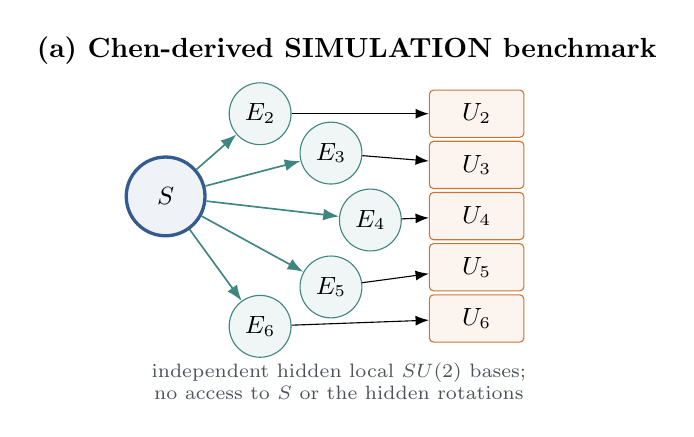
\begin{tikzpicture}[font=\sffamily\small,>=Latex,
 ph/.style={circle,draw=envteal,fill=envteal!8,minimum size=7.5mm},
 hid/.style={rounded corners=1.5pt,draw=accentorange,fill=accentorange!8,minimum width=12mm,minimum height=6mm,align=center}]
\node[font=\bfseries] at (2.9,2.35) {(a) Chen-derived SIMULATION benchmark};
\node[circle,draw=sysblue,very thick,fill=sysblue!8,minimum size=10mm] (S) at (.6,.5) {$S$};
\node[ph] (E2) at (1.8,1.55) {$E_2$};
\node[ph] (E3) at (2.7,1.05) {$E_3$};
\node[ph] (E4) at (3.2,.2) {$E_4$};
\node[ph] (E5) at (2.7,-.65) {$E_5$};
\node[ph] (E6) at (1.8,-1.15) {$E_6$};
\foreach \E in {E2,E3,E4,E5,E6}{\draw[->,semithick,draw=envteal] (S)--(\E);}
\node[hid] (u2) at (4.55,1.55) {$U_2$};
\node[hid] (u3) at (4.55,.90) {$U_3$};
\node[hid] (u4) at (4.55,.25) {$U_4$};
\node[hid] (u5) at (4.55,-.40) {$U_5$};
\node[hid] (u6) at (4.55,-1.05) {$U_6$};
\draw[->] (E2)--(u2); \draw[->] (E3)--(u3); \draw[->] (E4)--(u4); \draw[->] (E5)--(u5); \draw[->] (E6)--(u6);
\node[font=\scriptsize,align=center,text=deepgray] at (2.8,-1.85) {independent hidden local $SU(2)$ bases;\\no access to $S$ or the hidden rotations};
\end{tikzpicture}
\end{minipage}\hfill
\begin{minipage}{0.54\textwidth}
\centering
{\bfseries\color{accentred} SIMULATION}\par\vspace{0.4mm}
\includegraphics[width=\linewidth]{fig7_simulation_benchmark.pdf}
\end{minipage}
\caption{External hidden-readout simulation stress test.  (a) The record architecture follows the six-photon Quantum-Darwinism experiment of Chen \emph{et al.}, but each environmental photon is independently conjugated by an unknown local $SU(2)$ rotation before readout.  (b) In simulation, the learned decoder remains close to the physical oracle floor in both the all-strong-record and mixed strong/weak-record settings.  This is a benchmark derived from the published architecture, not a reanalysis of raw experimental events.}
\label{fig:chen}
\end{figure*}

\subsection{Operational resource tradeoff}


A task-specific pair-moment implementation of Theorem~\ref{thm:binary-helstrom} estimates local binary decoder axes from environment-environment correlations.  For five fragments, an orthogonal-array Pauli schedule uses 27 distinct environment-only settings; a stronger specialized baseline with direct access to $S$ uses 9 settings; full six-qubit Pauli tomography uses 729.  At equal total copy budget in the Chen-derived simulation, environment-only and system-assisted methods have comparable decoder-axis errors.  The conclusion is therefore not a universal resource advantage.  The tradeoff is operational: removing direct system access can be achieved without full-state reconstruction, at the cost of additional environmental measurements relative to a specialized system-assisted protocol.

\begin{figure*}[t]
\centering
\begin{minipage}{0.48\textwidth}
\centering
\includegraphics[width=\linewidth]{fig8a_equal_budget.pdf}
\end{minipage}\hfill
\begin{minipage}{0.48\textwidth}
\centering
\includegraphics[width=\linewidth]{fig8b_settings_scaling.pdf}
\end{minipage}
\caption{Task-specific resource benchmark retained from the earlier EIQL study.  Left: decoder-axis error at equal total copy budget for an environment-only pair-moment estimator and a stronger system-assisted correlation baseline.  Right: distinct measurement-setting counts.  The comparison demonstrates an access tradeoff, not a universal sample-complexity advantage.}
\label{fig:resource}
\end{figure*}

\section{Discussion}

The analysis sharpens the EIQL interpretation in three ways.  The earlier agreement-richness objective is retained in Appendix~\ref{app:agreement} as a practical heuristic with a documented failure boundary, not as a foundational identification principle.

First, redundancy is not merely an agreement signal.  In product-record models it changes the geometry of the inverse problem: response overlaps and support coherences multiply across fragments.  This can improve robust rank and, in rank-deficient branching models, create support transversality.  However, more redundancy is not automatically better for full state reconstruction because product spectra can become poorly conditioned.  Decoder learning can therefore be substantially easier than latent-state tomography.

Second, there is no universal fragment count.  Two fragments suffice for equal-prior binary Helstrom decoding, but Proposition~\ref{prop:unequal-prior} shows that even a known unequal prior can restore ambiguity.  Pairwise data can also suffice in structured SBS-like multiclass regimes, whereas generic multiclass common-support records can require a third view for full latent identification.  The relevant question is not simply ``how many fragments?'' but ``which object is being identified, what prior structure is known, and what geometry do the records have?''

Third, structural identifiability and semantics are distinct.  Even perfect reconstruction of a latent environmental record does not prove that the latent variable is a property of the designated system.  The passive no-go theorem makes this unavoidable.  Physics enters through trusted causal structure: a known interaction model, a system preparation interface, or an intervention whose target is controlled.  The four-way intervention tensor provides one constructive route.

The theory remains conditional on branching or related low-order latent structure.  Non-Markovian environments, inter-fragment interactions, and scrambling can violate those assumptions \cite{galve2016,duruisseau2023}.  The new numerical suite probes two such practical boundaries---finite sampling and a controlled conditional-correlation defect---and the microscopic collision model verifies that the estimator can be driven from microscopic $S$--$E$ dynamics rather than analytically inserted record states.  These checks do not remove the structural assumptions: they cover a restricted perturbation family and a small qubit model.  The finite-shot binary theorem gives a closed-form concentration bound, but its snapshot constants can scale strongly with fragment dimension, and the generic multiclass finite-sample theory still inherits conditioning requirements from robust tensor decomposition.  The SBS spectral construction likewise requires operator-level estimation of $\sigma_B$ and $K_B$ and is not asserted to be measurement-cheap in generic dimension.  All present validation remains simulation-only; neither the Chen-derived benchmark nor the readout-noise and collision studies are calibrated to a specific device.  These limitations preclude claims of broad experimental self-calibration.

The resulting interpretation is therefore modest but concrete.  Quantum Darwinism explains why the environment can become a public witness.  EIQL asks when an observer can infer how that witness should be read.  Readability, statistical identifiability, and causal semantics are different layers of that task.

\section{Conclusion}

We formulated unknown environmental readout as an identifiability problem downstream of Quantum Darwinism.  Three conclusions carry the central contribution.  First, unknown-readout identifiability is hierarchical: the recoverable object and the number of required views depend on the prior and on the geometry of the environmental records.  Second, redundancy is not only a carrier of repeated information; in product-record models it can improve inverse conditioning by suppressing response overlap and support coherence, even when full-state spectral conditioning does not improve.  Third, structural recovery and semantics are distinct: passive environmental observations cannot universally certify that a recovered latent variable is a record of the designated system, whereas a trusted intervention can provide the missing causal anchor.

The numerical studies support these conclusions at finite resources through binary finite-shot scaling, controlled model mismatch, multiclass two-view ambiguity and three-view recovery, and a microscopic collision-model phase boundary.  They are operational stress tests rather than hardware validation.  The resulting question is therefore narrower than Quantum Darwinism, SBS, tensor learning, or tomography individually: under what physical and statistical conditions can redundant environmental records reveal a usable readout, and what extra causal information is required before that readout can be assigned system-specific meaning?

\section*{Data Availability}
No external or proprietary datasets were used.  The numerical data shown in the figures are generated from the analytical models and simulation procedures described in the manuscript.  Reproducibility scripts and generated numerical tables are maintained in the accompanying public repository at \url{https://github.com/AHDMarwan/Environment-Induced-Quantum-Learning}, including the finite-shot binary study, conditional-correlation stress test, multiclass two-versus-three-view experiment, microscopic collision-model phase diagram, near-SBS and conditioning checks, Chen-derived simulation benchmark, resource comparison, and algebraic counterexamples.  The Chen-derived benchmark uses the published experimental architecture only; it does not use raw experimental events.


\clearpage
\section*{References}
\begin{thebibliography}{99}
\footnotesize

\bibitem{wootters1982} W. K. Wootters and W. H. Zurek, A single quantum cannot be cloned, \emph{Nature} \textbf{299}, 802 (1982).
\bibitem{barnum1996} H. Barnum, C. M. Caves, C. A. Fuchs, R. Jozsa, and B. Schumacher, Noncommuting mixed states cannot be broadcast, \emph{Phys. Rev. Lett.} \textbf{76}, 2818 (1996).
\bibitem{zurek2003} W. H. Zurek, Decoherence, einselection, and the quantum origins of the classical, \emph{Rev. Mod. Phys.} \textbf{75}, 715 (2003).
\bibitem{ollivier2004} H. Ollivier, D. Poulin, and W. H. Zurek, Objective properties from subjective quantum states: Environment as a witness, \emph{Phys. Rev. Lett.} \textbf{93}, 220401 (2004).
\bibitem{ollivier2005} H. Ollivier, D. Poulin, and W. H. Zurek, Environment as a witness: Selective proliferation of information and emergence of objectivity in a quantum universe, \emph{Phys. Rev. A} \textbf{72}, 042113 (2005).

\bibitem{zurek2009} W. H. Zurek, Quantum Darwinism, \emph{Nat. Phys.} \textbf{5}, 181 (2009).
\bibitem{zurek2022} W. H. Zurek, Quantum theory of the classical: Einselection, envariance, Quantum Darwinism and extantons, \emph{Entropy} \textbf{24}, 1520 (2022).
\bibitem{zurek2025book} W. H. Zurek, \emph{Decoherence and Quantum Darwinism: From Quantum Foundations to Classical Reality} (Cambridge University Press, Cambridge, 2025).
\bibitem{korbicz2014} J. K. Korbicz, P. Horodecki, and R. Horodecki, Objectivity in a noisy photonic environment through quantum state information broadcasting, \emph{Phys. Rev. Lett.} \textbf{112}, 120402 (2014).
\bibitem{horodecki2015} R. Horodecki, J. K. Korbicz, and P. Horodecki, Quantum origins of objectivity, \emph{Phys. Rev. A} \textbf{91}, 032122 (2015).
\bibitem{brandao2015} F. G. S. L. Brand\~ao, M. Piani, and P. Horodecki, Generic emergence of classical features in quantum Darwinism, \emph{Nat. Commun.} \textbf{6}, 7908 (2015).
\bibitem{le2019} T. P. Le and A. Olaya-Castro, Strong Quantum Darwinism and strong independence are equivalent to spectrum broadcast structure, \emph{Phys. Rev. Lett.} \textbf{122}, 010403 (2019).
\bibitem{korbicz2021} J. K. Korbicz, Roads to objectivity: Quantum Darwinism, spectrum broadcast structures, and strong quantum Darwinism--a review, \emph{Quantum} \textbf{5}, 571 (2021).
\bibitem{fu2021} H.-F. Fu, Uniqueness of the observable leaving redundant imprints in the environment in the context of Quantum Darwinism, \emph{Phys. Rev. A} \textbf{103}, 042210 (2021).
\bibitem{touil2022} A. Touil, B. Yan, D. Girolami, S. Deffner, and W. H. Zurek, Eavesdropping on the decohering environment: Quantum Darwinism, amplification, and the origin of objective classical reality, \emph{Phys. Rev. Lett.} \textbf{128}, 010401 (2022).
\bibitem{girolami2022} D. Girolami, A. Touil, B. Yan, S. Deffner, and W. H. Zurek, Redundantly amplified information suppresses quantum correlations in many-body systems, \emph{Phys. Rev. Lett.} \textbf{129}, 010401 (2022).
\bibitem{touil2024branch} A. Touil, F. Anza, S. Deffner, and J. P. Crutchfield, Branching states as the emergent structure of a quantum universe, \emph{Quantum} \textbf{8}, 1494 (2024).
\bibitem{touil2025} A. Touil, B. Yan, and W. H. Zurek, Consensus about classical reality in a quantum universe, arXiv:2503.14791 (2025).
\bibitem{doucet2025} E. Doucet and S. Deffner, Compatibility of quantum measurements and the emergence of classical objectivity, \emph{Phys. Rev. A} \textbf{111}, 042217 (2025).
\bibitem{kiely2026} A. Kiely, D. A. Chisholm, A. Touil, S. Deffner, G. Landi, and S. Campbell, Metrological approach to the emergence of classical objectivity, \emph{Phys. Rev. A} \textbf{113}, 022403 (2026).
\bibitem{torvinen2026} J. Torvinen, E. Keski-Vakkuri, and N. Pranzini, Quantum Darwinism and the quality of Petz recovery, arXiv:2605.06848 (2026).
\bibitem{alfsen2012} E. Alfsen and F. Shultz, Finding decompositions of a class of separable states, arXiv:1202.3673 (2012).
\bibitem{allman2009} E. S. Allman, C. Matias, and J. A. Rhodes, Identifiability of parameters in latent structure models with many observed variables, \emph{Ann. Stat.} \textbf{37}, 3099 (2009).
\bibitem{anandkumar2014} A. Anandkumar, R. Ge, D. Hsu, S. M. Kakade, and M. Telgarsky, Tensor decompositions for learning latent variable models, \emph{J. Mach. Learn. Res.} \textbf{15}, 2773 (2014).
\bibitem{bhaskara2014} A. Bhaskara, M. Charikar, and A. Vijayaraghavan, Uniqueness of tensor decompositions with applications to polynomial identifiability, in \emph{Proc. 26th ACM-SIAM Symposium on Discrete Algorithms} (2014), arXiv:1304.8087.
\bibitem{sidiropoulos2017} N. D. Sidiropoulos, L. De Lathauwer, X. Fu, K. Huang, E. E. Papalexakis, and C. Faloutsos, Tensor decomposition for signal processing and machine learning, \emph{IEEE Trans. Signal Process.} \textbf{65}, 3551 (2017).
\bibitem{helstrom1976} C. W. Helstrom, \emph{Quantum Detection and Estimation Theory} (Academic Press, New York, 1976).
\bibitem{fuchscaves1996} C. A. Fuchs and C. M. Caves, Mathematical techniques for quantum communication theory, \emph{Open Syst. Inf. Dyn.} \textbf{3}, 345 (1995); arXiv:quant-ph/9604001.
\bibitem{fuchsvandegraaf1999} C. A. Fuchs and J. van de Graaf, Cryptographic distinguishability measures for quantum-mechanical states, \emph{IEEE Trans. Inf. Theory} \textbf{45}, 1216 (1999).
\bibitem{huang2020} H.-Y. Huang, R. Kueng, and J. Preskill, Predicting many properties of a quantum system from very few measurements, \emph{Nat. Phys.} \textbf{16}, 1050 (2020).
\bibitem{stephens2021} A. Stephens, J. M. Cutshall, T. McPhee, and M. Beck, Self-consistent state and measurement tomography with fewer measurements, \emph{Phys. Rev. A} \textbf{104}, 012416 (2021).
\bibitem{cattaneo2023} M. Cattaneo, M. A. C. Rossi, K. Korhonen, E.-M. Borrelli, G. Garc\'ia-P\'erez, Z. Zimbor\'as, and D. Cavalcanti, Self-consistent quantum measurement tomography based on semidefinite programming, \emph{Phys. Rev. Research} \textbf{5}, 033154 (2023).
\bibitem{chen2019} M.-C. Chen, H.-S. Zhong, Y. Li, D. Wu, X.-L. Wang, L. Li, N.-L. Liu, C.-Y. Lu, and J.-W. Pan, Emergence of classical objectivity of Quantum Darwinism in a photonic quantum simulator, \emph{Sci. Bull.} \textbf{64}, 580 (2019).
\bibitem{zhu2025} Z. Zhu \emph{et al.}, Observation of quantum Darwinism and the origin of classicality with superconducting circuits, \emph{Sci. Adv.} \textbf{11}, eadx6857 (2025).
\bibitem{galve2016} F. Galve, R. Zambrini, and S. Maniscalco, Non-Markovianity hinders Quantum Darwinism, \emph{Sci. Rep.} \textbf{6}, 19607 (2016).
\bibitem{duruisseau2023} P. Duruisseau, A. Touil, and S. Deffner, Pointer states and Quantum Darwinism with two-body interactions, \emph{Entropy} \textbf{25}, 1573 (2023).

\end{thebibliography}

\clearpage
\appendix

\section{Proof details}
\label{app:proofs}

\subsection{Proof of Theorem~\ref{thm:subspace}}
Vectorize Hermitian operators in a real Hilbert-Schmidt basis and define
\begin{equation}
A_i=[\sqrt{p_1}|\delta_{i,1}\rangle\!\rangle,\ldots,\sqrt{p_r}|\delta_{i,r}\rangle\!\rangle],
\end{equation}
with analogous $A_j$.  Eq.~\eqref{eq:multi-connected} corresponds to $A_iA_j^\top$.  Because $A_i\sqrt p=A_j\sqrt p=0$, where $\sqrt p=(\sqrt{p_1},\ldots,\sqrt{p_r})^\top$, and both matrices have rank $r-1$, each nullspace is exactly $\Span\{\sqrt p\}$.  Therefore $\operatorname{range}(A_j^\top)=(\sqrt p)^\perp$, and the restriction of $A_i$ to that subspace maps onto $\operatorname{range}(A_i)=\cS_i$.  Hence $\operatorname{range}(A_iA_j^\top)=\cS_i$.  The right-support statement is symmetric.

\subsection{Finite-shot concentration for Theorem~\ref{thm:finite-binary}}
Within each physical realization, $(R_i,R_j)$ is a same-event snapshot pair, so $\mathbb E[R_i\otimes R_j]$ retains the desired two-fragment correlation. Let $(R_i',R_j')$ be an independent second realization. Then
\begin{align}
&\mathbb E[(R_i-R_i')\otimes(R_j-R_j')]\notag\\
&\qquad=2\mathbb E[R_i\otimes R_j]-2\mathbb E[R_i]\otimes\mathbb E[R_j],
\end{align}
which proves unbiasedness after the factor $1/2$. Set
\begin{equation}
K_s=\frac12(R_i^{2s-1}-R_i^{2s})\otimes(R_j^{2s-1}-R_j^{2s}).
\end{equation}
The snapshot bounds imply
\begin{equation}
\|K_s\|_2\le \frac12(2B_i)(2B_j)=2B_iB_j=:L.
\end{equation}
For the Hilbert-space empirical mean $Z=N^{-1}\sum_s(K_s-\mathbb EK_s)$, independence gives
\begin{equation}
\mathbb E\|Z\|_2^2
=\frac1{N^2}\sum_s\mathbb E\|K_s-\mathbb EK_s\|_2^2
\le\frac{L^2}{N},
\end{equation}
so $\mathbb E\|Z\|_2\le L/\sqrt N$. Replacing one pair changes $\|Z\|_2$ by at most $2L/N$. McDiarmid therefore yields, with probability at least $1-\beta$,
\begin{equation}
\|Z\|_2\le\frac{L}{\sqrt N}
\left[1+\sqrt{2\ln(1/\beta)}\right],
\end{equation}
which is Eq.~\eqref{eq:finite-omega} because $L=2B_iB_j$. Wedin's rank-one bound gives
\begin{equation}
\sin\theta\le\frac{e_N}{\lambda-e_N}.
\end{equation}
Requiring this to be at most $\varepsilon$ is equivalent to $e_N\le\varepsilon\lambda/(1+\varepsilon)$. Substituting $\lambda=\|\Delta_i\|_2\|\Delta_j\|_2/4$ and converting from $N$ independent pairs to $n=2N$ physical events gives the factor $128$ in Eq.~\eqref{eq:finite-binary-n}. This independently checks both the bounded-difference constant and the pair-to-event conversion.

\subsection{Proof of Theorem~\ref{thm:response-conditioning}}

The Gram matrix $G_B=\widetilde A_B^\top\widetilde A_B$ has diagonal entries one and off-diagonal entries bounded by $\mu_B$.  Gershgorin's theorem places all eigenvalues in
\begin{equation}
[1-(r-1)\mu_B,\,1+(r-1)\mu_B].
\end{equation}
The singular-value statement follows because the eigenvalues of $G_B$ are the squared singular values of $\widetilde A_B$.  For a subset of $q$ columns, the corresponding principal Gram matrix has the same unit diagonal and off-diagonal bound $\mu_B$, so Gershgorin gives $1-(q-1)\mu_B$ and proves Corollary~\ref{cor:subset-conditioning}.

\subsection{Proof of Theorem~\ref{thm:support-transverse}}
For $v_x\in V_x$,
\begin{equation}
|\langle v_x,v_{x'}\rangle|
\le\|P_xP_{x'}\|_\infty\|v_x\|\|v_{x'}\|
\le c\|v_x\|\|v_{x'}\|.
\end{equation}
Expanding $\|\sum_xv_x\|^2$ and using
\begin{equation}
2\sum_{x<x'}a_xa_{x'}\le(r-1)\sum_xa_x^2
\end{equation}
gives Eq.~\eqref{eq:support-frame}.

\subsection{Marginal eigenvalue bound}
Write $\beta_{\mathcal B,x}=R_xR_x^\dagger$ on its support, with $\sigma_{\min}(R_x)^2\ge b_{\mathcal B}$.  Define
\begin{equation}
F(z_1,\ldots,z_r)=\sum_x\sqrt{p_x}R_xz_x.
\end{equation}
Then $\rho_B=FF^\dagger$.  The support-transversality theorem applied to $w_x=\sqrt{p_x}R_xz_x$ gives
\begin{equation}
\|Fz\|^2\ge[1-(r-1)c_{\mathcal B}]p_{\min}b_{\mathcal B}\|z\|^2,
\end{equation}
which proves Eq.~\eqref{eq:marginal-conditioning}.

\subsection{Robust spectral anchor}
Let $X=\sigma_B^{-1/2}$ and $\widehat X=\rho_B^{-1/2}$ on the ideal occupied support. If $\sigma_B\ge mI$ and $\|\rho_B-\sigma_B\|_\infty\le\eps<m/2$, then $\rho_B\ge mI/2$, so
\begin{equation}
\|X\|_\infty\le m^{-1/2},
\qquad
\|\widehat X\|_\infty\le\sqrt{2/m}.
\end{equation}
The integral representation
\begin{equation}
A^{-1/2}=\frac1\pi\int_0^\infty t^{-1/2}(A+tI)^{-1}\,dt
\end{equation}
and the resolvent identity imply, on the interval $[m/2,\infty)$,
\begin{equation}
\|\widehat X-X\|_\infty
\le\frac{\sqrt2\,\eps}{m^{3/2}}
=:d_X.
\end{equation}
Because $\|H_A\|_\infty\le1$, one has $-\sigma_B\le K_B\le\sigma_B$ and likewise for the perturbed state; in particular $\|K_B\|_\infty,\|\widehat K_B\|_\infty\le1$. Moreover,
\begin{equation}
\|\widehat K_B-K_B\|_\infty\le\eps.
\end{equation}
Expand
\begin{align}
\widehat L_B-L_B
={}&(\widehat X-X)\widehat K_B\widehat X
+X(\widehat K_B-K_B)\widehat X\notag\\
&+XK_B(\widehat X-X).
\end{align}
Therefore
\begin{align}
\|\widehat L_B-L_B\|_\infty
&\le d_X\sqrt{2/m}
+\frac{\eps}{\sqrt m}\sqrt{2/m}
+\frac{d_X}{\sqrt m}\notag\\
&=\frac{\sqrt2\,\eps}{m}
+\frac{(2+\sqrt2)\eps}{m^2},
\end{align}
which is Eq.~\eqref{eq:sbs-perturb}. If the distinct ideal eigenvalue clusters are separated by $g$ and $\eta_{\rm SBS}<g/2$, the Hermitian Davis--Kahan theorem yields Eq.~\eqref{eq:projector-bound}. The displayed $m^{-1}$ and $m^{-2}$ deterioration is therefore a whitening-conditioning effect rather than an unspecified perturbation constant.

\section{Exact multiclass pairwise counterexample}
\label{app:counterexample}

Let the conditional commuting states on $A$ and $B$ be represented by column-stochastic matrices
\begin{equation}
U=\begin{pmatrix}
3/5&1/5&1/5\\
3/10&3/5&1/5\\
1/10&1/5&3/5
\end{pmatrix},\quad
V=\begin{pmatrix}
1/2&1/5&3/10\\
3/10&1/2&1/5\\
1/5&3/10&1/2
\end{pmatrix},
\end{equation}
with $p=(3/10,3/10,2/5)$.  The observed two-view distribution is
\begin{equation}
P=U\diag(p)V^\top
=\begin{pmatrix}
63/500&1/10&47/500\\
21/200&133/1000&14/125\\
99/1000&87/1000&18/125
\end{pmatrix}.
\end{equation}
The same $P$ admits
\begin{equation}
p'=(39/200,81/200,2/5),
\end{equation}
\begin{align}
U'&=\begin{pmatrix}
3/5&41/135&1/5\\
3/10&47/90&1/5\\
1/10&47/270&3/5
\end{pmatrix},\\[1mm]
V'&=\begin{pmatrix}
43/65&1/5&3/10\\
5/26&1/2&1/5\\
19/130&3/10&1/2
\end{pmatrix}.
\end{align}
The two decompositions are not related by a common permutation.  For the first ensemble, the optimal local MAP decision on the computational-basis outcome of $A$ is $(0,1,2)$; for the second it is $(1,1,2)$.  The accompanying script verifies $\|P-P'\|_{\max}<1.4\times10^{-17}$ in double precision.

\section{Earlier agreement-richness guarantee}
\label{app:agreement}

For completeness, we record the output-level theorem used by the earlier EIQL objective.  Let $Z_1,\ldots,Z_m\in\cZ$, $|\cZ|=L$, and define
\begin{equation}
D=\max_{i<j}P(Z_i\neq Z_j),\qquad
R=\min_jH(Z_j).
\end{equation}
Let
\begin{equation}
\xi_{ij}=\sum_xp_x\TV\left(P_{Z_iZ_j|x},P_{Z_i|x}P_{Z_j|x}\right),
\qquad
\xi=\max_{i<j}\xi_{ij}.
\end{equation}
If $D\le\epsilon$, $R\ge H(X)-\kappa$, and $\xi\le\alpha$, define $\delta=\epsilon+\alpha$.  For $\delta\le1-1/L$, each fragment admits a deterministic $g_j(X)$ with
\begin{equation}
P[Z_j\neq g_j(X)]\le\delta
\end{equation}
and
\begin{equation}
H(X|Z_j)\le\kappa+h_2(\delta)+\delta\log_2(L-1).
\end{equation}
For a cq state with $\nu=\max_{i<j}I(E_i:E_j|X)$ bits, data processing and Pinsker give $\alpha\le\sqrt{(\ln2)\nu/2}$ for the post-measurement total-variation defect.  This theorem is conditional on a system-referenced common-cause model and does not self-certify that the common record is about $S$.

For a fixed finite candidate class of size $Q$, Hoeffding and a union bound provide a uniform finite-shot certificate.  At the earlier numerical operating point $Q=500$, $m=4$, $L=2$, $n=600$, and failure probability $0.05$, the disagreement deviation bound is $0.1016$ and the entropy-continuity penalty is $0.4777$ bit, making the resulting worst-case certificate effectively vacuous at a target disagreement of $0.10$.  This is why the present paper replaces the generic finite-class theorem, where possible, by geometry-dependent results such as Theorem~\ref{thm:finite-binary}.

\section{Reproducibility notes}

The ancillary reproducibility bundle contains the scripts and numerical tables used for the unequal-prior binary counterexample, finite-shot Theorem~\ref{thm:finite-binary} study, conditional-correlation stress test, exact multiclass counterexample and three-view recovery experiment, microscopic five-fragment collision-model phase diagram, near-SBS spectral-anchor check, support-geometry checks, and conditioning stress test.  The Chen-derived and resource-comparison figures are simulation outputs from the earlier EIQL study.  No private experimental data are used.  The Chen benchmark is based on the published architecture and hidden local-basis simulations; the fidelity-proxy and noise studies in the earlier version are not reconstructions of the laboratory channel.



\end{document}
